\chapter{Introduction}\label{ch:intro}

In this chapter we are going to describe accurately the problem and provide a possible 
solution (from the point of view of a Distributed Systems designer).\\


\section{The Problem}

The bridge has a \textbf{maximum capacity} $c \geq 1$ and a certain length $l$. 

Cars can send messages to adjacent cars (to the car in front and to the rear one); 
cars can also have the ability to speak with more than two other cars depending on the 
\textbf{power of their transmission medium} $p \geq 1$.

The initialization of a communication between two cars can be done unsing an 
\textbf{environment process} 
that returns the required references needed to start the message exchange.

So basically a car can only send messages to the $p$ cars in front and 
to the $p$ cars behind. We assume that \textbf{the bridge length doesn't 
constitute an impediment}
for the communications (so even if the bridge was very long, however, 
the cars can send messages as if they were close).

By default every car has the same dimensions (but can be setted to an arbitrary
\textbf{size}) expressed in a custom length scale called \textbf{block} and 
\textbf{every measure is an integer} ($l$, $c$, $p$, etc.). \\

\noindent
We assume that cars can have a failure at any moment and there are only 
three types of failures:
\begin{itemize}
    \item \textbf{mechanical failure} (the car cannot move but can send messages to the other cars)
    \item \textbf{link failure} (the car can move but cannot send any message)
    \item \textbf{system failure} (the car cannot move and cannot send messages)
\end{itemize}

\noindent
We assume that a link failure is equivalent to a system failure cause the car cannot 
take any decision without the agreement of the others. 

In case of engine failure or system failure the car or another helping car must call 
a tow truck in order to remove the broken car 
(in this case we have to wait an \textbf{elimination time} $e$).

In case of failure the car behind has to wait until the tow truck removes the broken car.\\

\noindent
We assume that a car cannot be malicius (must follow the algorithm) but the communication 
channel isn't secure so it is exposed to a \textbf{MIM} (man in the middle) attack 
(drop messages, edit messages, message injection, ...).\\

\noindent
Finally we have to consider that in a distributed system a global up-to-date state 
or a global timing cannot exist; this implies that each car can have a partial 
and \textbf{inconsistent view} of the global environment and a \textbf{time drift} 
from the global time (for this reason the system cannot guarantee the FIFO ordering 
at all).

\begin{figure}[h]
    \centering
    \resizebox{12cm}{5cm}{%
    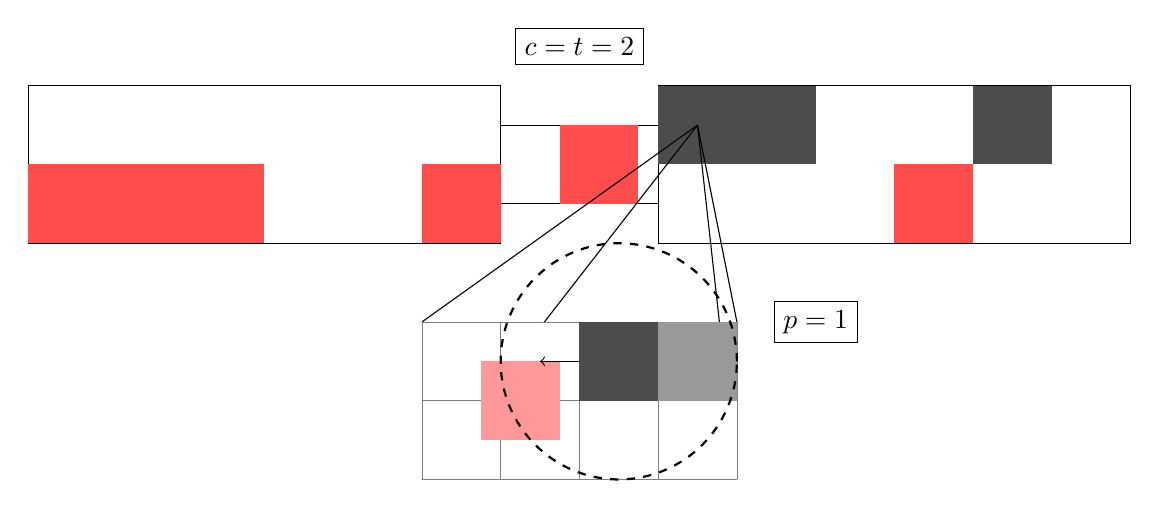
\begin{tikzpicture}
        % queues
        \draw (1,-1) rectangle (7,1);
        \draw (-7,-1) rectangle (-1,1);
        
        % bridge
        \draw (-1,-0.5) rectangle (1,0.5);
        \fill[red!70!white] (-0.25,-0.5) rectangle (0.75,0.5);
        \fill[red!70!white] (4,-1) rectangle (5,0);
        \node[draw,align=left] at (0,1.5) {$c = t = 2 $};
        
        % left cars
        \fill[red!70!white] (-7,-1) rectangle (-6,0);
        \fill[red!70!white] (-6,-1) rectangle (-5,0);
        \fill[red!70!white] (-5,-1) rectangle (-4,0);
        \fill[red!70!white] (-2,-1) rectangle (-1,0);
        
        %% right cars
        \fill[black!70!white] (1,0) rectangle (2,1);
        \fill[black!70!white] (2,0) rectangle (3,1);
        \fill[black!70!white] (5,0) rectangle (6,1);
        
        \draw[black] (1.5,0.5) -- (-2, -2);
        \draw[black] (1.5,0.5) -- (2, -2);
        \draw[black] (1.5,0.5) -- (-2, -4);
        \draw[black] (1.5,0.5) -- (2, -4);

        % grid
        \fill[white]  (-2,-4) rectangle (2, -2);
        \draw[step=1cm,gray,very thin] (-2,-4) grid (2, -2);
        \fill[black!70!white] (0,-3) rectangle (1,-2);
        \fill[black!40!white] (1,-3) rectangle (2,-2);
        \fill[red!40!white] (-1.25,-3.5) rectangle (-0.25,-2.5);

        \draw[black,thick,dashed] (0.5,-2.5) circle (1.5cm);
        \node[draw,align=left] at (3,-2) {$p = 1$};
        \draw[->,black] (0,-2.5) -- (-0.5, -2.5);
    \end{tikzpicture}
    }
    \caption{Example of a possible situation} \label{fig:1}
\end{figure}


\section{Requirements}

The main requirements to be met are:
\begin{itemize}
    \item \textbf{Fairness}
    \item \textbf{Fault tolerance}
    \item \textbf{Without starvation}
    \item \textbf{Without deadlock}
\end{itemize}